\documentclass{article}
\usepackage{iclr2027_conference,times}
\iclrfinalcopy % camera-ready layout (no line numbers, author shown); running header blanked below
%%%%% NEW MATH DEFINITIONS %%%%%

\usepackage{amsmath,amsfonts,bm}

% Mark sections of captions for referring to divisions of figures
\newcommand{\figleft}{{\em (Left)}}
\newcommand{\figcenter}{{\em (Center)}}
\newcommand{\figright}{{\em (Right)}}
\newcommand{\figtop}{{\em (Top)}}
\newcommand{\figbottom}{{\em (Bottom)}}
\newcommand{\captiona}{{\em (a)}}
\newcommand{\captionb}{{\em (b)}}
\newcommand{\captionc}{{\em (c)}}
\newcommand{\captiond}{{\em (d)}}

% Highlight a newly defined term
\newcommand{\newterm}[1]{{\bf #1}}


% Figure reference, lower-case.
\def\figref#1{figure~\ref{#1}}
% Figure reference, capital. For start of sentence
\def\Figref#1{Figure~\ref{#1}}
\def\twofigref#1#2{figures \ref{#1} and \ref{#2}}
\def\quadfigref#1#2#3#4{figures \ref{#1}, \ref{#2}, \ref{#3} and \ref{#4}}
% Section reference, lower-case.
\def\secref#1{section~\ref{#1}}
% Section reference, capital.
\def\Secref#1{Section~\ref{#1}}
% Reference to two sections.
\def\twosecrefs#1#2{sections \ref{#1} and \ref{#2}}
% Reference to three sections.
\def\secrefs#1#2#3{sections \ref{#1}, \ref{#2} and \ref{#3}}
% Reference to an equation, lower-case.
\def\eqref#1{equation~\ref{#1}}
% Reference to an equation, upper case
\def\Eqref#1{Equation~\ref{#1}}
% A raw reference to an equation---avoid using if possible
\def\plaineqref#1{\ref{#1}}
% Reference to a chapter, lower-case.
\def\chapref#1{chapter~\ref{#1}}
% Reference to an equation, upper case.
\def\Chapref#1{Chapter~\ref{#1}}
% Reference to a range of chapters
\def\rangechapref#1#2{chapters\ref{#1}--\ref{#2}}
% Reference to an algorithm, lower-case.
\def\algref#1{algorithm~\ref{#1}}
% Reference to an algorithm, upper case.
\def\Algref#1{Algorithm~\ref{#1}}
\def\twoalgref#1#2{algorithms \ref{#1} and \ref{#2}}
\def\Twoalgref#1#2{Algorithms \ref{#1} and \ref{#2}}
% Reference to a part, lower case
\def\partref#1{part~\ref{#1}}
% Reference to a part, upper case
\def\Partref#1{Part~\ref{#1}}
\def\twopartref#1#2{parts \ref{#1} and \ref{#2}}

\def\ceil#1{\lceil #1 \rceil}
\def\floor#1{\lfloor #1 \rfloor}
\def\1{\bm{1}}
\newcommand{\train}{\mathcal{D}}
\newcommand{\valid}{\mathcal{D_{\mathrm{valid}}}}
\newcommand{\test}{\mathcal{D_{\mathrm{test}}}}

\def\eps{{\epsilon}}


% Random variables
\def\reta{{\textnormal{$\eta$}}}
\def\ra{{\textnormal{a}}}
\def\rb{{\textnormal{b}}}
\def\rc{{\textnormal{c}}}
\def\rd{{\textnormal{d}}}
\def\re{{\textnormal{e}}}
\def\rf{{\textnormal{f}}}
\def\rg{{\textnormal{g}}}
\def\rh{{\textnormal{h}}}
\def\ri{{\textnormal{i}}}
\def\rj{{\textnormal{j}}}
\def\rk{{\textnormal{k}}}
\def\rl{{\textnormal{l}}}
% rm is already a command, just don't name any random variables m
\def\rn{{\textnormal{n}}}
\def\ro{{\textnormal{o}}}
\def\rp{{\textnormal{p}}}
\def\rq{{\textnormal{q}}}
\def\rr{{\textnormal{r}}}
\def\rs{{\textnormal{s}}}
\def\rt{{\textnormal{t}}}
\def\ru{{\textnormal{u}}}
\def\rv{{\textnormal{v}}}
\def\rw{{\textnormal{w}}}
\def\rx{{\textnormal{x}}}
\def\ry{{\textnormal{y}}}
\def\rz{{\textnormal{z}}}

% Random vectors
\def\rvepsilon{{\mathbf{\epsilon}}}
\def\rvtheta{{\mathbf{\theta}}}
\def\rva{{\mathbf{a}}}
\def\rvb{{\mathbf{b}}}
\def\rvc{{\mathbf{c}}}
\def\rvd{{\mathbf{d}}}
\def\rve{{\mathbf{e}}}
\def\rvf{{\mathbf{f}}}
\def\rvg{{\mathbf{g}}}
\def\rvh{{\mathbf{h}}}
\def\rvu{{\mathbf{i}}}
\def\rvj{{\mathbf{j}}}
\def\rvk{{\mathbf{k}}}
\def\rvl{{\mathbf{l}}}
\def\rvm{{\mathbf{m}}}
\def\rvn{{\mathbf{n}}}
\def\rvo{{\mathbf{o}}}
\def\rvp{{\mathbf{p}}}
\def\rvq{{\mathbf{q}}}
\def\rvr{{\mathbf{r}}}
\def\rvs{{\mathbf{s}}}
\def\rvt{{\mathbf{t}}}
\def\rvu{{\mathbf{u}}}
\def\rvv{{\mathbf{v}}}
\def\rvw{{\mathbf{w}}}
\def\rvx{{\mathbf{x}}}
\def\rvy{{\mathbf{y}}}
\def\rvz{{\mathbf{z}}}

% Elements of random vectors
\def\erva{{\textnormal{a}}}
\def\ervb{{\textnormal{b}}}
\def\ervc{{\textnormal{c}}}
\def\ervd{{\textnormal{d}}}
\def\erve{{\textnormal{e}}}
\def\ervf{{\textnormal{f}}}
\def\ervg{{\textnormal{g}}}
\def\ervh{{\textnormal{h}}}
\def\ervi{{\textnormal{i}}}
\def\ervj{{\textnormal{j}}}
\def\ervk{{\textnormal{k}}}
\def\ervl{{\textnormal{l}}}
\def\ervm{{\textnormal{m}}}
\def\ervn{{\textnormal{n}}}
\def\ervo{{\textnormal{o}}}
\def\ervp{{\textnormal{p}}}
\def\ervq{{\textnormal{q}}}
\def\ervr{{\textnormal{r}}}
\def\ervs{{\textnormal{s}}}
\def\ervt{{\textnormal{t}}}
\def\ervu{{\textnormal{u}}}
\def\ervv{{\textnormal{v}}}
\def\ervw{{\textnormal{w}}}
\def\ervx{{\textnormal{x}}}
\def\ervy{{\textnormal{y}}}
\def\ervz{{\textnormal{z}}}

% Random matrices
\def\rmA{{\mathbf{A}}}
\def\rmB{{\mathbf{B}}}
\def\rmC{{\mathbf{C}}}
\def\rmD{{\mathbf{D}}}
\def\rmE{{\mathbf{E}}}
\def\rmF{{\mathbf{F}}}
\def\rmG{{\mathbf{G}}}
\def\rmH{{\mathbf{H}}}
\def\rmI{{\mathbf{I}}}
\def\rmJ{{\mathbf{J}}}
\def\rmK{{\mathbf{K}}}
\def\rmL{{\mathbf{L}}}
\def\rmM{{\mathbf{M}}}
\def\rmN{{\mathbf{N}}}
\def\rmO{{\mathbf{O}}}
\def\rmP{{\mathbf{P}}}
\def\rmQ{{\mathbf{Q}}}
\def\rmR{{\mathbf{R}}}
\def\rmS{{\mathbf{S}}}
\def\rmT{{\mathbf{T}}}
\def\rmU{{\mathbf{U}}}
\def\rmV{{\mathbf{V}}}
\def\rmW{{\mathbf{W}}}
\def\rmX{{\mathbf{X}}}
\def\rmY{{\mathbf{Y}}}
\def\rmZ{{\mathbf{Z}}}

% Elements of random matrices
\def\ermA{{\textnormal{A}}}
\def\ermB{{\textnormal{B}}}
\def\ermC{{\textnormal{C}}}
\def\ermD{{\textnormal{D}}}
\def\ermE{{\textnormal{E}}}
\def\ermF{{\textnormal{F}}}
\def\ermG{{\textnormal{G}}}
\def\ermH{{\textnormal{H}}}
\def\ermI{{\textnormal{I}}}
\def\ermJ{{\textnormal{J}}}
\def\ermK{{\textnormal{K}}}
\def\ermL{{\textnormal{L}}}
\def\ermM{{\textnormal{M}}}
\def\ermN{{\textnormal{N}}}
\def\ermO{{\textnormal{O}}}
\def\ermP{{\textnormal{P}}}
\def\ermQ{{\textnormal{Q}}}
\def\ermR{{\textnormal{R}}}
\def\ermS{{\textnormal{S}}}
\def\ermT{{\textnormal{T}}}
\def\ermU{{\textnormal{U}}}
\def\ermV{{\textnormal{V}}}
\def\ermW{{\textnormal{W}}}
\def\ermX{{\textnormal{X}}}
\def\ermY{{\textnormal{Y}}}
\def\ermZ{{\textnormal{Z}}}

% Vectors
\def\vzero{{\bm{0}}}
\def\vone{{\bm{1}}}
\def\vmu{{\bm{\mu}}}
\def\vtheta{{\bm{\theta}}}
\def\va{{\bm{a}}}
\def\vb{{\bm{b}}}
\def\vc{{\bm{c}}}
\def\vd{{\bm{d}}}
\def\ve{{\bm{e}}}
\def\vf{{\bm{f}}}
\def\vg{{\bm{g}}}
\def\vh{{\bm{h}}}
\def\vi{{\bm{i}}}
\def\vj{{\bm{j}}}
\def\vk{{\bm{k}}}
\def\vl{{\bm{l}}}
\def\vm{{\bm{m}}}
\def\vn{{\bm{n}}}
\def\vo{{\bm{o}}}
\def\vp{{\bm{p}}}
\def\vq{{\bm{q}}}
\def\vr{{\bm{r}}}
\def\vs{{\bm{s}}}
\def\vt{{\bm{t}}}
\def\vu{{\bm{u}}}
\def\vv{{\bm{v}}}
\def\vw{{\bm{w}}}
\def\vx{{\bm{x}}}
\def\vy{{\bm{y}}}
\def\vz{{\bm{z}}}

% Elements of vectors
\def\evalpha{{\alpha}}
\def\evbeta{{\beta}}
\def\evepsilon{{\epsilon}}
\def\evlambda{{\lambda}}
\def\evomega{{\omega}}
\def\evmu{{\mu}}
\def\evpsi{{\psi}}
\def\evsigma{{\sigma}}
\def\evtheta{{\theta}}
\def\eva{{a}}
\def\evb{{b}}
\def\evc{{c}}
\def\evd{{d}}
\def\eve{{e}}
\def\evf{{f}}
\def\evg{{g}}
\def\evh{{h}}
\def\evi{{i}}
\def\evj{{j}}
\def\evk{{k}}
\def\evl{{l}}
\def\evm{{m}}
\def\evn{{n}}
\def\evo{{o}}
\def\evp{{p}}
\def\evq{{q}}
\def\evr{{r}}
\def\evs{{s}}
\def\evt{{t}}
\def\evu{{u}}
\def\evv{{v}}
\def\evw{{w}}
\def\evx{{x}}
\def\evy{{y}}
\def\evz{{z}}

% Matrix
\def\mA{{\bm{A}}}
\def\mB{{\bm{B}}}
\def\mC{{\bm{C}}}
\def\mD{{\bm{D}}}
\def\mE{{\bm{E}}}
\def\mF{{\bm{F}}}
\def\mG{{\bm{G}}}
\def\mH{{\bm{H}}}
\def\mI{{\bm{I}}}
\def\mJ{{\bm{J}}}
\def\mK{{\bm{K}}}
\def\mL{{\bm{L}}}
\def\mM{{\bm{M}}}
\def\mN{{\bm{N}}}
\def\mO{{\bm{O}}}
\def\mP{{\bm{P}}}
\def\mQ{{\bm{Q}}}
\def\mR{{\bm{R}}}
\def\mS{{\bm{S}}}
\def\mT{{\bm{T}}}
\def\mU{{\bm{U}}}
\def\mV{{\bm{V}}}
\def\mW{{\bm{W}}}
\def\mX{{\bm{X}}}
\def\mY{{\bm{Y}}}
\def\mZ{{\bm{Z}}}
\def\mBeta{{\bm{\beta}}}
\def\mPhi{{\bm{\Phi}}}
\def\mLambda{{\bm{\Lambda}}}
\def\mSigma{{\bm{\Sigma}}}

% Tensor
\DeclareMathAlphabet{\mathsfit}{\encodingdefault}{\sfdefault}{m}{sl}
\SetMathAlphabet{\mathsfit}{bold}{\encodingdefault}{\sfdefault}{bx}{n}
\newcommand{\tens}[1]{\bm{\mathsfit{#1}}}
\def\tA{{\tens{A}}}
\def\tB{{\tens{B}}}
\def\tC{{\tens{C}}}
\def\tD{{\tens{D}}}
\def\tE{{\tens{E}}}
\def\tF{{\tens{F}}}
\def\tG{{\tens{G}}}
\def\tH{{\tens{H}}}
\def\tI{{\tens{I}}}
\def\tJ{{\tens{J}}}
\def\tK{{\tens{K}}}
\def\tL{{\tens{L}}}
\def\tM{{\tens{M}}}
\def\tN{{\tens{N}}}
\def\tO{{\tens{O}}}
\def\tP{{\tens{P}}}
\def\tQ{{\tens{Q}}}
\def\tR{{\tens{R}}}
\def\tS{{\tens{S}}}
\def\tT{{\tens{T}}}
\def\tU{{\tens{U}}}
\def\tV{{\tens{V}}}
\def\tW{{\tens{W}}}
\def\tX{{\tens{X}}}
\def\tY{{\tens{Y}}}
\def\tZ{{\tens{Z}}}


% Graph
\def\gA{{\mathcal{A}}}
\def\gB{{\mathcal{B}}}
\def\gC{{\mathcal{C}}}
\def\gD{{\mathcal{D}}}
\def\gE{{\mathcal{E}}}
\def\gF{{\mathcal{F}}}
\def\gG{{\mathcal{G}}}
\def\gH{{\mathcal{H}}}
\def\gI{{\mathcal{I}}}
\def\gJ{{\mathcal{J}}}
\def\gK{{\mathcal{K}}}
\def\gL{{\mathcal{L}}}
\def\gM{{\mathcal{M}}}
\def\gN{{\mathcal{N}}}
\def\gO{{\mathcal{O}}}
\def\gP{{\mathcal{P}}}
\def\gQ{{\mathcal{Q}}}
\def\gR{{\mathcal{R}}}
\def\gS{{\mathcal{S}}}
\def\gT{{\mathcal{T}}}
\def\gU{{\mathcal{U}}}
\def\gV{{\mathcal{V}}}
\def\gW{{\mathcal{W}}}
\def\gX{{\mathcal{X}}}
\def\gY{{\mathcal{Y}}}
\def\gZ{{\mathcal{Z}}}

% Sets
\def\sA{{\mathbb{A}}}
\def\sB{{\mathbb{B}}}
\def\sC{{\mathbb{C}}}
\def\sD{{\mathbb{D}}}
% Don't use a set called E, because this would be the same as our symbol
% for expectation.
\def\sF{{\mathbb{F}}}
\def\sG{{\mathbb{G}}}
\def\sH{{\mathbb{H}}}
\def\sI{{\mathbb{I}}}
\def\sJ{{\mathbb{J}}}
\def\sK{{\mathbb{K}}}
\def\sL{{\mathbb{L}}}
\def\sM{{\mathbb{M}}}
\def\sN{{\mathbb{N}}}
\def\sO{{\mathbb{O}}}
\def\sP{{\mathbb{P}}}
\def\sQ{{\mathbb{Q}}}
\def\sR{{\mathbb{R}}}
\def\sS{{\mathbb{S}}}
\def\sT{{\mathbb{T}}}
\def\sU{{\mathbb{U}}}
\def\sV{{\mathbb{V}}}
\def\sW{{\mathbb{W}}}
\def\sX{{\mathbb{X}}}
\def\sY{{\mathbb{Y}}}
\def\sZ{{\mathbb{Z}}}

% Entries of a matrix
\def\emLambda{{\Lambda}}
\def\emA{{A}}
\def\emB{{B}}
\def\emC{{C}}
\def\emD{{D}}
\def\emE{{E}}
\def\emF{{F}}
\def\emG{{G}}
\def\emH{{H}}
\def\emI{{I}}
\def\emJ{{J}}
\def\emK{{K}}
\def\emL{{L}}
\def\emM{{M}}
\def\emN{{N}}
\def\emO{{O}}
\def\emP{{P}}
\def\emQ{{Q}}
\def\emR{{R}}
\def\emS{{S}}
\def\emT{{T}}
\def\emU{{U}}
\def\emV{{V}}
\def\emW{{W}}
\def\emX{{X}}
\def\emY{{Y}}
\def\emZ{{Z}}
\def\emSigma{{\Sigma}}

% entries of a tensor
% Same font as tensor, without \bm wrapper
\newcommand{\etens}[1]{\mathsfit{#1}}
\def\etLambda{{\etens{\Lambda}}}
\def\etA{{\etens{A}}}
\def\etB{{\etens{B}}}
\def\etC{{\etens{C}}}
\def\etD{{\etens{D}}}
\def\etE{{\etens{E}}}
\def\etF{{\etens{F}}}
\def\etG{{\etens{G}}}
\def\etH{{\etens{H}}}
\def\etI{{\etens{I}}}
\def\etJ{{\etens{J}}}
\def\etK{{\etens{K}}}
\def\etL{{\etens{L}}}
\def\etM{{\etens{M}}}
\def\etN{{\etens{N}}}
\def\etO{{\etens{O}}}
\def\etP{{\etens{P}}}
\def\etQ{{\etens{Q}}}
\def\etR{{\etens{R}}}
\def\etS{{\etens{S}}}
\def\etT{{\etens{T}}}
\def\etU{{\etens{U}}}
\def\etV{{\etens{V}}}
\def\etW{{\etens{W}}}
\def\etX{{\etens{X}}}
\def\etY{{\etens{Y}}}
\def\etZ{{\etens{Z}}}

% The true underlying data generating distribution
\newcommand{\pdata}{p_{\rm{data}}}
% The empirical distribution defined by the training set
\newcommand{\ptrain}{\hat{p}_{\rm{data}}}
\newcommand{\Ptrain}{\hat{P}_{\rm{data}}}
% The model distribution
\newcommand{\pmodel}{p_{\rm{model}}}
\newcommand{\Pmodel}{P_{\rm{model}}}
\newcommand{\ptildemodel}{\tilde{p}_{\rm{model}}}
% Stochastic autoencoder distributions
\newcommand{\pencode}{p_{\rm{encoder}}}
\newcommand{\pdecode}{p_{\rm{decoder}}}
\newcommand{\precons}{p_{\rm{reconstruct}}}

\newcommand{\laplace}{\mathrm{Laplace}} % Laplace distribution

\newcommand{\E}{\mathbb{E}}
\newcommand{\Ls}{\mathcal{L}}
\newcommand{\R}{\mathbb{R}}
\newcommand{\emp}{\tilde{p}}
\newcommand{\lr}{\alpha}
\newcommand{\reg}{\lambda}
\newcommand{\rect}{\mathrm{rectifier}}
\newcommand{\softmax}{\mathrm{softmax}}
\newcommand{\sigmoid}{\sigma}
\newcommand{\softplus}{\zeta}
\newcommand{\KL}{D_{\mathrm{KL}}}
\newcommand{\Var}{\mathrm{Var}}
\newcommand{\standarderror}{\mathrm{SE}}
\newcommand{\Cov}{\mathrm{Cov}}
% Wolfram Mathworld says $L^2$ is for function spaces and $\ell^2$ is for vectors
% But then they seem to use $L^2$ for vectors throughout the site, and so does
% wikipedia.
\newcommand{\normlzero}{L^0}
\newcommand{\normlone}{L^1}
\newcommand{\normltwo}{L^2}
\newcommand{\normlp}{L^p}
\newcommand{\normmax}{L^\infty}

\newcommand{\parents}{Pa} % See usage in notation.tex. Chosen to match Daphne's book.

\DeclareMathOperator*{\argmax}{arg\,max}
\DeclareMathOperator*{\argmin}{arg\,min}

\DeclareMathOperator{\sign}{sign}
\DeclareMathOperator{\Tr}{Tr}
\let\ab\allowbreak

\usepackage{hyperref}
\hypersetup{colorlinks=true,linkcolor=black!70!blue,citecolor=black!60!green,urlcolor=black!70!blue}
\usepackage{url}
\usepackage{amsmath,amssymb,amsthm}
\usepackage{graphicx}
\usepackage{booktabs}
\usepackage{xcolor}
\usepackage{subcaption}
\usepackage[capitalize,noabbrev]{cleveref}
% Every reported number lives here, generated from results/full by scripts/make_numbers.py
% (plus the hand-computed full-scale additions at the end).  \prov{} would mark provisional values; none remain.
\newif\ifprov \provtrue
\newcommand{\prov}[1]{\ifprov\textcolor{blue}{#1}\else#1\fi}

% ---- scale of the study
\newcommand{\nDGPhone}{390}         % H1 DGPs (pilot: 40 easy + 36 hard); full: 390
\newcommand{\nDGPhard}{180}
\newcommand{\nReps}{20}

% ---- H1: easy suite
\newcommand{\kEasyRic}{0.948}      \newcommand{\kEasyRicCI}{[0.938, 0.955]}
\newcommand{\kEasyOv}{0.993}       \newcommand{\kEasyOvCI}{[0.983, 1.002]}
% ---- H1: hard suite
\newcommand{\kHardPFN}{0.604}      \newcommand{\kHardPFNCI}{[0.574, 0.635]}
\newcommand{\kHardGP}{0.740}       \newcommand{\kHardGPCI}{[0.708, 0.771]}
\newcommand{\kHardAIPW}{0.616}     \newcommand{\kHardIPW}{0.603}
\newcommand{\kHardOLS}{0.439}
\newcommand{\dPFNGP}{$-0.135$}     \newcommand{\dPFNGPCI}{[$-0.145$, $-0.125$]}
\newcommand{\dPFNAIPW}{$-0.012$}   \newcommand{\dPFNAIPWCI}{[$-0.025$, $+0.002$]}
% ---- H1: positivity control
\newcommand{\kClipPFN}{0.675}      \newcommand{\kClipPFNCI}{[0.635, 0.715]}
\newcommand{\kClipIPW}{0.852}
\newcommand{\dClipPFNIPW}{$-0.177$} \newcommand{\dClipPFNIPWCI}{[$-0.250$, $-0.106$]}
\newcommand{\trendHard}{$-0.033$}  \newcommand{\trendClip}{$-0.013$}
\newcommand{\regP}{$-0.010$} 
\newcommand{\regLogN}{$+0.127$}
% ---- H2
\newcommand{\linRemoved}{89\%}     \newcommand{\nonlinRemoved}{32\%}
\newcommand{\nonlinShareLeft}{79\%}
\newcommand{\corrKappaNonlin}{$-0.905$}
\newcommand{\hajekBetter}{61\%}    \newcommand{\negWeights}{20\%}
\newcommand{\corrInvE}{n/a}
\newcommand{\cosFresh}{0.47--0.81} \newcommand{\labelDep}{7.2\%}
\newcommand{\cosHOin}{0.54} \newcommand{\cosSRA}{0.98}
% ---- H3
\newcommand{\nHthree}{35}
\newcommand{\probeReal}{0.73}  \newcommand{\probeShuf}{0.55}
\newcommand{\probeRand}{0.61}  \newcommand{\probeRawx}{0.38}
\newcommand{\shufDrop}{0.18}
\newcommand{\eraseOne}{0.104}  \newcommand{\eraseOneUB}{0.132}
\newcommand{\eraseAll}{0.239}  \newcommand{\eraseAllUB}{0.287}
\newcommand{\eraseNuis}{0.051} \newcommand{\eraseRand}{0.007}
% ---- IHDP (filled after run_ihdp.py)
\newcommand{\ihdpA}{0.944} \newcommand{\ihdpB}{1.008}
% ---- IHDP balance attribution (run_ihdp.py, 15 surfaces per setting)
\newcommand{\ihdpGPA}{0.983} \newcommand{\ihdpGPB}{0.961}
\newcommand{\ihdpNonlinShare}{5\%}
\newcommand{\ihdpLinLeftPFN}{0.089} \newcommand{\ihdpLinLeftGP}{0.032}
% ---- full-scale additions (Kaggle run, 22 Nov 2026)
\newcommand{\kHardGPfull}{0.740} \newcommand{\kHardHO}{0.502} \newcommand{\dHOS}{$-0.102$}
\newcommand{\kClipGP}{0.784} \newcommand{\dClipPFNGP}{$-0.108$} \newcommand{\dClipPFNGPCI}{[$-0.122$, $-0.095$]}
\newcommand{\kClipAIPW}{0.722}
\newcommand{\dPFNIPWhard}{$+0.001$} \newcommand{\dPFNIPWhardCI}{[$-0.018$, $+0.020$]}
\newcommand{\clipHigher}{88/90}
\newcommand{\corrEVChard}{0.87} \newcommand{\corrEVCclip}{0.95}
\newcommand{\kInPrior}{0.993} \newcommand{\kOutPrior}{0.948}
\newcommand{\dEasyGPric}{$-0.036$}
\newcommand{\gpLin}{87\%} \newcommand{\gpNonlin}{51\%}
\newcommand{\olsNonlin}{$-48\%$} \newcommand{\hajLin}{91\%} \newcommand{\hajNonlin}{95\%}
\newcommand{\corrKappaLin}{$-0.59$}
\newcommand{\cosPFNGP}{0.55} \newcommand{\cosPFNOLS}{0.46} \newcommand{\cosPFNHaj}{0.36}
\newcommand{\cosGPFresh}{0.87} \newcommand{\cosPFNFresh}{0.66}
\newcommand{\attnReal}{0.48} \newcommand{\attnShuf}{0.31} \newcommand{\attnRand}{0.22} \newcommand{\attnLayers}{12 of 20}
\newcommand{\swapGP}{1.18} \newcommand{\swapGPCI}{[0.73, 1.99]} \newcommand{\swapIPW}{0.05} \newcommand{\swapIPWCI}{[$-0.02$, 0.11]}
\newcommand{\swapAbsPFN}{0.082} \newcommand{\swapAbsGP}{0.034} \newcommand{\swapAbsIPW}{0.275} \newcommand{\swapAbsErased}{0.105}
\newcommand{\eraseLogit}{0.77}


\newtheorem{proposition}{Proposition}
\newcommand{\DiM}{\mathrm{DiM}}
\newcommand{\that}{\hat\tau}
\newcommand{\todo}[1]{\textcolor{red}{[TODO: #1]}}

\title{What Estimator Does CausalPFN Learn?\\An Exact Weighting View of\\a Causal Foundation Model}

\author{Pranav Kalla}

\begin{document}
\maketitle
\lhead{}\renewcommand{\headrulewidth}{0pt}

\begin{abstract}
Causal foundation models such as CausalPFN estimate treatment effects in a single forward pass, but it is unknown how they correct for confounding. We show that CausalPFN's per-arm outcome standardisation makes its average-treatment-effect estimate \emph{exactly} a weighting estimator, $\that = \DiM + \sum_i w^{\mathrm{net}}_i y_i$, and that its error equals the imbalance of these weights on the true outcome surfaces plus a noise term. Across \nDGPhone{} synthetic data-generating processes, IHDP, probes, LEACE erasure and coupled propensity swaps, we find three things. (i)~CausalPFN removes nearly all confounding bias in low-dimensional problems, but only \kHardPFN{} of it under dense, weak, nonlinear confounding, against \kHardGP{} for a Gaussian-process S-learner given the same preprocessing. The gap persists when overlap is bounded. (ii)~The implied weights remove \linRemoved{} of the linear but only \nonlinRemoved{} of the nonlinear confounding. \nonlinShareLeft{} of the remaining bias is nonlinear, and its size predicts the shortfall ($r={}$\corrKappaNonlin). (iii)~Propensity information is computed in the context-row representations from the first layer and is partly used: erasing it moves the estimate by \eraseOne{}--\eraseAll{} of the correction. Yet when only the propensity changes, CausalPFN responds like the GP outcome model, not like inverse-propensity weighting. CausalPFN thus behaves as a regularised outcome smoother whose balance is essentially linear. This locates the failure that recent debiasing methods target. Code and results: \url{https://github.com/PRANAVKALLA230106/causalpfn-weighting}.
\end{abstract}

\section{Introduction}
Prior-data fitted networks (PFNs) amortise Bayesian inference over a synthetic prior \citep{muller2022pfn,hollmann2023tabpfn}. Causal variants, including CausalPFN \citep{balazadeh2025causalpfn}, Do-PFN \citep{robertson2025dopfn} and CausalFM \citep{ma2025causalfm}, estimate conditional and average treatment effects from a table in one forward pass \citep{stith2026cfmsurvey}. Their behaviour is increasingly well mapped. They retain prior-driven bias that can prevent frequentist consistency \citep{melnychuk2026frequentist}, a cousin of regularisation-induced confounding \citep{hahn2018regularization}, and they degrade with post-treatment covariates \citep{ham2026posttreatment}. Several works propose fixes that change the training target or add a correction step \citep{melnychuk2026frequentist,zhang2026fluctuate}. Internal analyses exist only for tabular \emph{prediction} models \citep{bilos2026mechanistic,nguyen2026standardization,gupta2026tabpfnheads,gong2026depth}. No one has asked where, inside a causal foundation model, the confounding correction is computed or lost.

\paragraph{Contributions.}
\begin{enumerate}
\item \textbf{An exact weighting representation} of CausalPFN's ATE (\cref{prop:weights}), from per-arm $z$-scoring and Euler's theorem. Its \emph{error identity} attributes estimation error to the imbalance of the implied weights on the true outcome surfaces, which we split into linear and nonlinear parts.
\item \textbf{How much correction?} Near-complete in low-dimensional sparse problems. Under dense nonlinear confounding, the correction falls with dimension and rises with $n$, and stays below a GP S-learner with identical preprocessing, also when overlap is bounded (\cref{sec:h1}).
\item \textbf{What is balanced?} The weights balance the linear span of $X$ almost as well as oracle inverse-propensity weights do, and its nonlinear complement far worse. The nonlinear residual predicts the shortfall (\cref{sec:h2}). On IHDP, confounding is almost entirely linear, so this failure mode never shows (\cref{sec:ihdp}).
\item \textbf{Where is propensity?} Probes with shuffled-treatment and random-network controls, LEACE erasure \citep{belrose2023leace}, attention analysis and coupled propensity swaps show that propensity is computed and partly used, but that CausalPFN responds to propensity changes like an outcome model (\cref{sec:h3}).
\end{enumerate}
Code, all result files and the scripts that regenerate every number and figure are available at \url{https://github.com/PRANAVKALLA230106/causalpfn-weighting}.

\section{Setup}\label{sec:setup}
\paragraph{Estimand and the share of bias removed.}
We observe $(x_i, t_i, y_i)_{i=1}^n$ with $t_i\in\{0,1\}$, $n_1$ treated and $n_0$ controls, and outcome surfaces $\mu_t(x)$. The sample effect is $\psi = n^{-1}\sum_i[\mu_1(x_i)-\mu_0(x_i)]$, and $\DiM = \bar y_1 - \bar y_0$. For a data-generating process (DGP) $d$ we define the share of confounding bias removed by an estimator $\that$ as
\begin{equation}
\kappa_d = \frac{\mathbb{E}[\that - \DiM]}{\mathbb{E}[\psi - \DiM]},
\end{equation}
with expectations over replications that redraw $(X, T, \varepsilon)$. $\kappa=0$ is DiM; $\kappa=1$ for any consistent estimator. We use only DGPs whose DiM bias exceeds three Monte-Carlo standard errors. We report $|\text{bias}|$-weighted pooled $\kappa$ with DGP-clustered bootstrap 95\% intervals, and compare estimators \emph{paired} on identical draws.

\paragraph{CausalPFN's computation.}
CausalPFN standardises outcomes \emph{per arm}, $z_i = (y_i - \bar y_{t_i})/s_{t_i}$, with population standard deviations. A transformer reads context tokens $(x_i, t_i, z_i)$ and outputs standardised conditional expected potential outcomes $m_t(x)$. These are mapped back as $\hat\mu_t(x) = \bar y_t + s_t\,m_t(x)$. The S-mode ATE averages $\hat\mu_1-\hat\mu_0$ over the training rows. RA mode replaces the factual prediction by the observed outcome. We also use a cross-fitted \emph{held-out} mode, where queries never duplicate a context row.

\begin{proposition}[Exact weighting and error identity]\label{prop:weights}
For S, RA and cross-fitted modes:
(a) $\that(c\,\mathbf y) = c\,\that(\mathbf y)$ for $c>0$, and $\that(\mathbf y + a\mathbf 1_{T} + b\mathbf 1_{C}) = \that(\mathbf y) + a - b$.
(b) Hence $\that = \sum_i w_i y_i$ with $w = \nabla_{\mathbf y}\that$, where $\sum_{i\in T} w_i = 1$ and $\sum_{i\in C} w_i = -1$. Writing $w = w^{\DiM} + w^{\mathrm{net}}$ with $w^{\DiM}_i = \pm 1/n_{t_i}$, $w^{\mathrm{net}}$ sums to zero within each arm, and $|\that - \DiM| \le v_{\max}(s_1+s_0)$ with $v_{\max}=10$ the output-grid bound.
(c) With $y_i = \mu_{t_i}(x_i) + \varepsilon_i$ and control weights $v_i = -w_i$,
\begin{equation}\label{eq:error}
\that - \psi = \Big[\textstyle\sum_{i\in T} w_i\mu_1(x_i) - \bar\mu_1\Big] - \Big[\sum_{i\in C} v_i\mu_0(x_i) - \bar\mu_0\Big] + \sum_i w_i\varepsilon_i ,
\end{equation}
where $\bar\mu_t = n^{-1}\sum_i \mu_t(x_i)$.
\end{proposition}
\begin{proof}[Proof sketch]
(a) $z$ is invariant to positive scaling and to arm-wise shifts. $\bar y_t$ and $s_t$ transform equivariantly. (b) Euler's theorem for degree-1 homogeneous functions gives $\that = \mathbf y^\top\nabla\that$ \citep[cf.][]{hesse2021fast}. Differentiating the shift identity in $a$ and $b$ gives the arm sums. The bound holds because $m_t \in [-v_{\max}, v_{\max}]$. (c) Substitute $y_i$ into $\that=\sum w_i y_i$ and use $\psi = \bar\mu_1-\bar\mu_0$ and the arm sums. Full proof in \cref{app:proof}.
\end{proof}
The weights depend on $\mathbf y$, so they describe CausalPFN \emph{locally}, consistent with joint label processing \citep{nguyen2026standardization}. \Cref{eq:error} is nonetheless exact at the observed data. All identities hold numerically to $\le 1.1\times10^{-15}$ in float64 across 570 decompositions, and our direct path reproduces the public estimator to $<10^{-6}$ on CPU and GPU (\cref{app:impl}). Splitting $\mu_t$ into its best linear fit $L_t$ and remainder $N_t$ splits the bias term in \cref{eq:error} into a \emph{linear} and a \emph{nonlinear} imbalance. The same split applies to any weighting estimator, including DiM, OLS, oracle Hájek and the GP S-learner, whose exact weights we also compute.

\section{Experimental design}\label{sec:design}
\paragraph{DGP families} (\cref{app:dgp}), sized by a pilot power analysis:
\begin{itemize}
\item \emph{Easy} (120 DGPs): low-dimensional ($p\in\{3,5,8\}$) sparse surfaces. In the RIC variant, propensity is a function of the prognostic score \citep{hahn2018regularization}; in the overlap variant, propensity is linear with heterogeneous effects.
\item \emph{Hard} (180 DGPs): a grid over $p\in\{5,\dots,50\}$, confounding strength $1$--$6$ and $n\in\{200,500,1000\}$ with dense, weak, nonlinear confounding. Every covariate enters $\mu_0$ with coefficient $\propto p^{-1/2}$, and $e(x)=\sigma(\text{strength}\cdot\text{standardised }\mu_0)$.
\item \emph{Clip} (90 DGPs): the same surfaces with $e\in[0.1,0.9]$, a positivity control.
\item \emph{Prop-NL} (40 DGPs, for H3): propensity nonlinear in two coordinates and only partly prognostic, so propensity information is separable from outcome information.
\item \emph{IHDP}: the real covariates and treatment of the IHDP study, with Hill's linear (A) and nonlinear (B) surfaces \citep{hill2011bayesian,louizos2017cevae}.
\end{itemize}
Every DGP has \nReps{} replications. Following the prior description of \citet{balazadeh2025causalpfn}, DGPs whose propensity is aligned with the prognostic score are labelled out-of-prior.

\paragraph{Baselines,} all run on identical draws: DiM, OLS S/T-learners, IPW, Hájek, five-fold cross-fitted AIPW, $k$NN matching, and a GP S-learner on per-arm standardised outcomes. The GP shares CausalPFN's preprocessing and isolates ``regularised smoother'' behaviour. All runs use the public checkpoint (18.8M parameters).

\section{How much of the correction does CausalPFN supply?}\label{sec:h1}
\paragraph{Easy DGPs.} CausalPFN is nearly complete: $\kappa=\kEasyRic$~\kEasyRicCI{} on RIC and \kEasyOv~\kEasyOvCI{} on overlap DGPs, both inside an equivalence band of $[0.9, 1.1]$. It is lower on the out-of-prior RIC family than on the in-prior overlap family (\kOutPrior{} vs \kInPrior), and \dEasyGPric{} behind the GP on RIC.

\paragraph{Hard DGPs.} CausalPFN removes \kHardPFN~\kHardPFNCI{} of the bias (\cref{fig:kappa}), against \kHardGP{} for the GP on the same draws, a paired gap of \dPFNGP~\dPFNGPCI. It matches IPW (\dPFNIPWhard~\dPFNIPWhardCI) and AIPW (\dPFNAIPW~\dPFNAIPWCI), which are themselves limited by propensities near 0 and 1.

\paragraph{Bounded overlap.} With overlap bounded to $[0.1,0.9]$, CausalPFN improves in \clipHigher{} DGPs but still reaches only \kClipPFN~\kClipPFNCI{}. It trails the GP (\kClipGP; paired \dClipPFNGP~\dClipPFNGPCI) and IPW (\kClipIPW; paired \dClipPFNIPW~\dClipPFNIPWCI).

\paragraph{Drivers.} Regressing $\kappa_d$ on design factors under bounded overlap gives effects of dimension (\regP{} per covariate) and sample size (\regLogN{} per $\log n$). The confounding-strength effect shrinks from \trendHard{} to \trendClip{} once overlap is bounded, so it is mostly a positivity effect. Across DGPs, $\kappa_d$ correlates \corrEVChard{} (hard) and \corrEVCclip{} (clip) with how much of the explainable held-out outcome variance CausalPFN captures. The correction is thus limited by how well the in-context outcome model fits. Held-out queries, which halve the context, lower $\kappa$ to \kHardHO{} (paired difference \dHOS).

\begin{figure}[t]
\centering
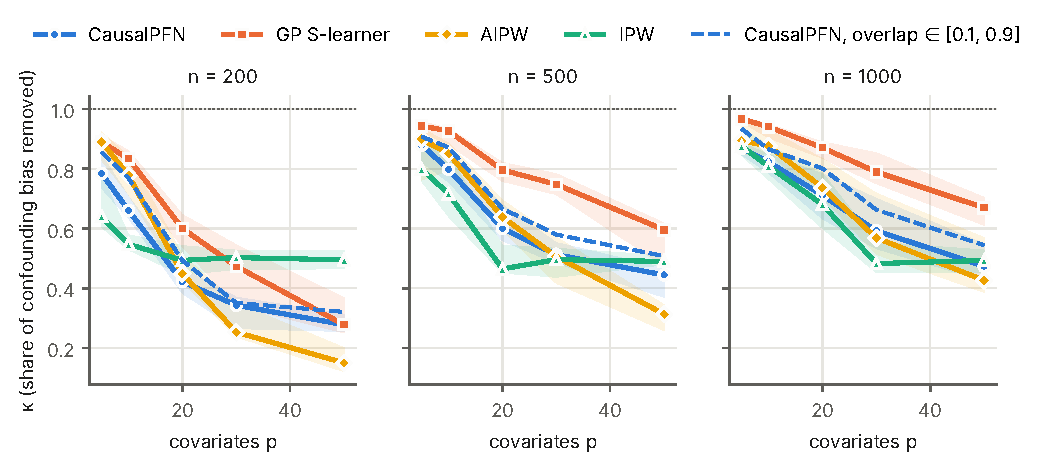
\includegraphics[width=\linewidth]{figures/fig1_kappa_vs_p.pdf}
\caption{Share of confounding bias removed ($\kappa$) on hard DGPs, by dimension and sample size (medians over DGPs, interquartile bands; 20 replications each). Dashed: CausalPFN on the same surfaces with overlap bounded to $[0.1,0.9]$.}
\label{fig:kappa}
\end{figure}

\section{What do the implied weights balance?}\label{sec:h2}
\Cref{eq:error} tells us which part of the outcome surface the weights fail to balance (\cref{fig:balance}). On hard DGPs, CausalPFN's exact weights remove \linRemoved{} of DiM's linear confounding but only \nonlinRemoved{} of its nonlinear confounding. At $p=50$, and at $p=30$ with $n\le 500$, they \emph{increase} the nonlinear imbalance. \nonlinShareLeft{} of CausalPFN's remaining bias is nonlinear, and $\kappa_d$ correlates \corrKappaNonlin{} with the residual nonlinear imbalance, against \corrKappaLin{} with the linear one. The reference estimators bracket this behaviour:
\begin{itemize}
\item OLS imputation balances the linear span exactly and worsens the nonlinear part (\olsNonlin), as regression-imputation theory predicts \citep{chattopadhyay2021implied,han2026imputation}.
\item Oracle Hájek weights balance both parts (\hajLin{} / \hajNonlin).
\item The GP sits between OLS and Hájek (\gpLin{} / \gpNonlin{}).
\end{itemize}
CausalPFN lies between OLS and the GP. Its weights are closest to the GP's: their within-arm cosine is \cosPFNGP, against \cosPFNOLS{} for OLS and \cosPFNHaj{} for oracle Hájek, and CausalPFN's own cosine under a fresh noise draw is \cosPFNFresh{} (\cref{app:extra}). \negWeights{} of its weights are negative, as for regression weights \citep{knaus2024weighted}. Oracle-free Hájek balances a rich covariate dictionary better than CausalPFN in \hajekBetter{} of datasets.

Two qualifications apply. First, the weights are local: the label-dependent chain-rule term is \labelDep{} of their norm, and the fresh-noise cosine ranges over \cosFresh. Second, held-out and in-context weights differ (cosine \cosHOin), so the duplicate own-row queries of S mode matter, whereas S and RA weights nearly coincide (\cosSRA).

\begin{figure}[t]
\centering
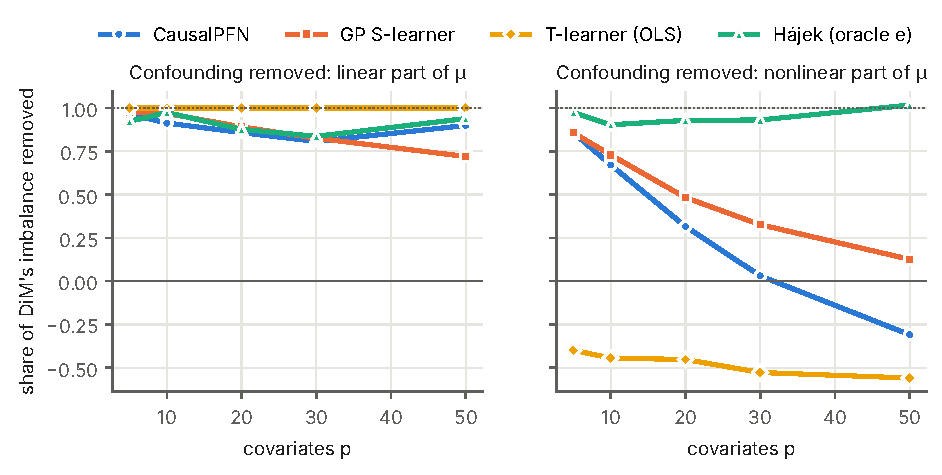
\includegraphics[width=0.9\linewidth]{figures/fig2_linear_vs_nonlinear_balance.pdf}
\caption{Share of DiM's imbalance removed on the linear and nonlinear parts of $\mu$ (\cref{eq:error}), for exact weights of each estimator, on hard DGPs (360 decompositions; averaged over $n$).}
\label{fig:balance}
\end{figure}

\subsection{A real-covariate check: IHDP}\label{sec:ihdp}
On IHDP's real covariates and treatment assignment (\cref{fig:ihdp}), CausalPFN removes most of the bias under both of Hill's surfaces: $\kappa=\ihdpA$ (linear surface A) and \ihdpB{} (nonlinear surface B), against \ihdpGPA{} and \ihdpGPB{} for the GP. \Cref{eq:error} explains why. Even under surface B, only \ihdpNonlinShare{} of DiM's imbalance falls on the nonlinear part of $\mu_0$, because the real assignment is aligned with the linear part. IHDP therefore never exercises the failure mode of \cref{fig:balance}, which suggests that standard semi-synthetic benchmarks can hide it. Where IHDP's confounding is linear, CausalPFN still leaves more linear imbalance than the GP (mean $|\cdot|$ \ihdpLinLeftPFN{} vs \ihdpLinLeftGP{} on surface A).

\begin{figure}[t]
\centering
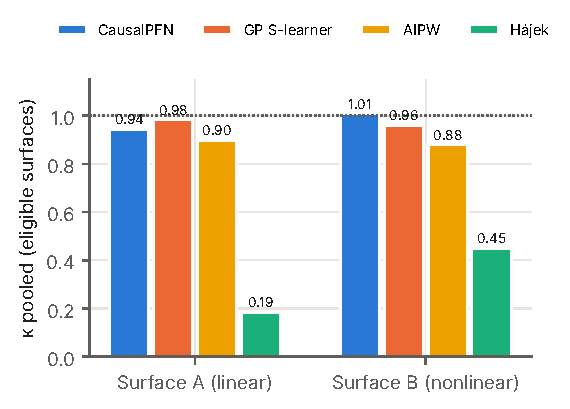
\includegraphics[width=0.52\linewidth]{figures/fig7_ihdp.pdf}
\caption{IHDP (real covariates and assignment; 40 surfaces per setting, 3 noise draws each): pooled $\kappa$ over surfaces with detectable DiM bias (32/40 for A, 20/40 for B).}
\label{fig:ihdp}
\end{figure}

\section{Where is propensity information, and is it used?}\label{sec:h3}
\paragraph{Probes.} We probe each layer's context-row stream for $e_\perp$, the logit propensity residualised on $(x, \mu_0(x), t)$, on \nHthree{} prop-NL DGPs. At the layer $l^*$ fixed on three pilot DGPs, $e_\perp$ is decodable with $R^2=\probeReal$. That exceeds a cubic polynomial of $x$ (\probeRawx), a random-init network (\probeRand) and the same network with $t$ shuffled across rows (\probeShuf). The shuffle drop (\shufDrop) appears for $e_\perp$ but not for a matched nuisance concept (\cref{fig:probes}, left), so CausalPFN computes propensity from the $t$--$x$ association.

\paragraph{Attention.} The attention mass that query rows place on treated context rows also tracks $\mathrm{logit}\,e$ beyond a quadratic in $x$ (mean max-head partial $|r|$ \attnReal, against \attnShuf{} with $t$ shuffled and \attnRand{} for a random network), in \attnLayers{} layers (\cref{app:extra}).

\paragraph{Erasure.} Decodability is not use \citep{belinkov2022probing,elazar2021amnesic}. LEACE erasure of $e_\perp$ moves $\that$ by \eraseOne{} of the correction at $l^*$ (90\% upper bound \eraseOneUB) and by \eraseAll{} (\eraseAllUB) when erased at every layer, against \eraseNuis{} for the nuisance concept and \eraseRand{} for random directions (\cref{fig:probes}, right). This exceeds our pre-registered 10\% margin, so the hypothesis that propensity is known but unused is \emph{falsified}: propensity carries a real, if minor, share of the correction.

\paragraph{Coupled propensity swaps.} To see \emph{how} it is used, we change only the propensity strength while holding $X$, $U$, $\varepsilon$ and the outcome surfaces fixed, so $\Delta\psi=0$. CausalPFN's change in estimate is predicted by the GP outcome model's change (coefficient \swapGP~\swapGPCI) and not by IPW's (\swapIPW~\swapIPWCI). Its mean $|\Delta\that|$ (\swapAbsPFN) lies between the GP's (\swapAbsGP) and IPW's (\swapAbsIPW), and grows to \swapAbsErased{} when $e_\perp$ is erased. Propensity information thus stabilises an estimate whose response to the assignment mechanism is that of an outcome model.

\begin{figure}[t]
\centering
\begin{subfigure}{0.49\linewidth}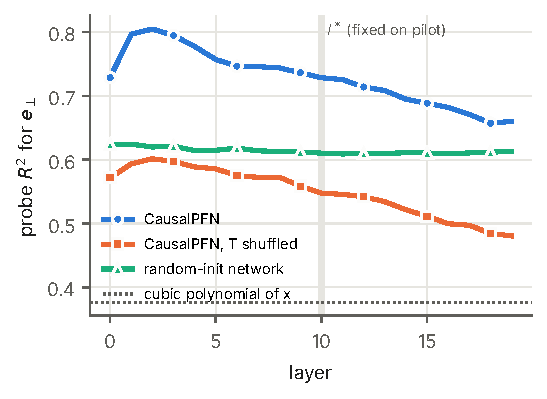
\includegraphics[width=\linewidth]{figures/fig4_propensity_probes.pdf}\end{subfigure}\hfill
\begin{subfigure}{0.49\linewidth}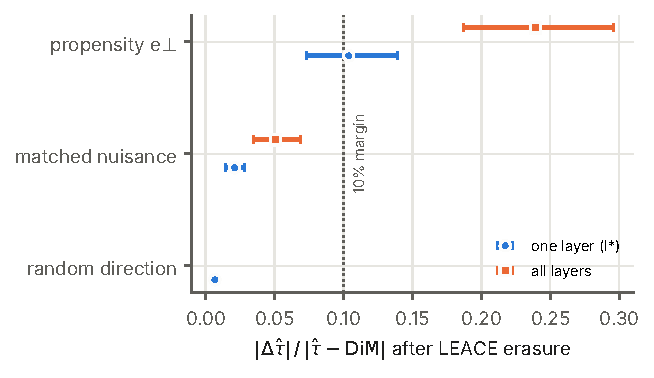
\includegraphics[width=\linewidth]{figures/fig5_erasure.pdf}\end{subfigure}
\caption{Left: probe $R^2$ for propensity-specific information $e_\perp$ by layer, with controls (\nHthree{} DGPs). Right: change in $\that$ after LEACE erasure, relative to the correction (bootstrap 95\% intervals; dotted: pre-registered 10\% margin).}
\label{fig:probes}
\end{figure}

\section{Related work}
\textbf{Causal foundation models}: \citet{balazadeh2025causalpfn,robertson2025dopfn,ma2025causalfm,stith2026cfmsurvey}. CInA links attention to covariate balancing \citep{zhang2023cina}. Their shrinkage and its fixes are studied in \citet{melnychuk2026frequentist,zhang2026fluctuate,ham2026posttreatment}. \textbf{Interpretability of tabular PFNs}: \citet{bilos2026mechanistic,gupta2026tabpfnheads,gong2026depth,shaheen2026generalization}. \citet{nguyen2026standardization} certify joint label processing and caution against derivatives taken after standardisation; our derivatives are taken \emph{before} standardisation, through it. \textbf{Estimators as weights}: \citet{chattopadhyay2021implied,knaus2024weighted,han2026imputation}. \textbf{Probing and erasure}: \citet{belinkov2022probing,elazar2021amnesic,belrose2023leace}.

\section{Discussion and limitations}
CausalPFN corrects for confounding as a regularised outcome smoother. Its implied weights balance the linear span of $X$ about as well as oracle inverse-propensity weights do, and nonlinear functions much worse. It computes propensity and uses it for a minor share of the correction, but its response to the assignment mechanism is that of an outcome model. This explains why its shortfall grows with dimension, shrinks with $n$ and tracks held-out fit. It also locates the failure that one-step corrections target \citep{melnychuk2026frequentist}: nonlinear imbalance. \Cref{eq:error} offers a practical diagnostic on simulated surrogates of one's data. The IHDP result cautions that standard benchmarks with near-linear confounding can hide the problem. Limitations: mostly synthetic DGPs (IHDP adds real covariates but only mild, near-linear confounding); one model; weights that are exact but local; and linear erasure, which bounds but does not exhaust propensity use.

\bibliography{refs}
\bibliographystyle{iclr2027_conference}

\appendix
\section{Proof of \cref{prop:weights}}\label{app:proof}
Let $\mathcal T, \mathcal C$ be the arms. For $c>0$, $\bar y_t(c\mathbf y) = c\bar y_t$, $s_t(c\mathbf y)=cs_t$ and $z(c\mathbf y)=z(\mathbf y)$. The network sees only $(x,t,z)$, so $m_t$ is unchanged and $\hat\mu_t(x; c\mathbf y) = c\hat\mu_t(x;\mathbf y)$. In RA mode, observed outcomes also scale by $c$. Hence $\that(c\mathbf y)=c\that(\mathbf y)$. (CausalPFN adds $10^{-20}$ to $s_t$; the induced deviation is below float64 resolution for all our data.) For the shift, $z$ is unchanged, $\bar y_1 \mapsto \bar y_1 + a$ and $\bar y_0\mapsto \bar y_0 + b$. Every $\hat\mu_1$ and every observed treated outcome moves by $a$, and every control quantity by $b$, so $\that$ moves by $a-b$. Euler's theorem for differentiable degree-1 homogeneous functions gives $\that = \sum_i y_i\,\partial\that/\partial y_i$. Differentiating $\that(\mathbf y + a\mathbf 1_{\mathcal T}) = \that(\mathbf y) + a$ in $a$ gives $\sum_{i\in\mathcal T}w_i = 1$; similarly $\sum_{i\in\mathcal C} w_i=-1$. For (c), $\that - \psi = \sum_{\mathcal T}w_i\mu_1(x_i) + \sum_{\mathcal C}w_i\mu_0(x_i) + \sum_i w_i\varepsilon_i - \bar\mu_1 + \bar\mu_0$. Rearranging with $v_i = -w_i$ on $\mathcal C$ gives \cref{eq:error}. In cross-fitted mode, each half-estimate is homogeneous in its own context outcomes, and the same argument applies to their average. \qed

\section{Implementation details}\label{app:impl}
\begin{itemize}
\item We call the network directly. With each arm at most 1{,}024 rows, CausalPFN's retrieval keeps every row, and the direct ATE matches \texttt{ATEEstimator.estimate\_ate} to $9\times10^{-8}$ (S) and $1.8\times10^{-7}$ (RA).
\item Exact decompositions run in float64. CausalPFN's RMSNorm casts to float32, which we patch to preserve dtype; this changes float32 predictions by $<10^{-6}$. Per-layer activation checkpointing gives bit-identical gradients.
\item The label-free/label-dependent split of $w^{\mathrm{net}}$ follows from the chain rule through $z$-scoring (population SD): with $G_k = \partial(s_1M_1 - s_0M_0)/\partial z_k$ at fixed $s$, we have $w^{\mathrm{net}}_j = (G_j - \bar G_a)/s_a + z_j(\sigma_a s_a M_a - \sum_{k\in a}G_kz_k)/(n_as_a)$ for $j$ in arm $a$. It holds to $10^{-17}$.
\end{itemize}
Full-scale runs used a Tesla T4 (PyTorch 2.11). On the same dataset, GPU and CPU agree to $2.4\times10^{-7}$ for $\that$ in float32 and to $2.8\times10^{-16}$ for the float64 weights. Six randomly chosen Kaggle rows recomputed on CPU agree to $\le 4.5\times10^{-7}$ for CausalPFN and exactly for the baselines.

\section{DGPs, prior labels and power analysis}\label{app:dgp}
All families draw $X\sim\mathcal N(0, I_p)$ afresh in every replication, set $T\sim\mathrm{Bernoulli}(e(X))$ with $e$ clipped to $[c, 1-c]$, and $Y = \mu_T(X) + \sigma\varepsilon$ with $\varepsilon\sim\mathcal N(0,1)$. Functional parameters are fixed per DGP by its seed.
\begin{itemize}
\item \textbf{Easy-RIC} ($p\in\{3,5,8\}$, $n=500$, $c=0.01$): $\mu_0(x) = \beta^\top x + a_1\sin(1.5x_1) + a_2(x_2^2-1) + a_3x_1x_3$, with $\beta$ 80\% dense; $\mu_1 = \mu_0 + \tau_0$, $|\tau_0|\le 0.3$; $e(x) = \sigma(s\cdot \tilde\mu_0(x))$, where $\tilde\mu_0$ is $\mu_0$ standardised over the population and $s\sim U(0.5,3)$.
\item \textbf{Easy-overlap}: same $\mu_0$; $\tau(x) = \tau_0 + \gamma_\tau^\top x$; $e(x) = \sigma(s\,\gamma^\top x)$ with $\gamma$ a unit vector on 1--3 coordinates and $s\sim U(1,4)$.
\item \textbf{Hard} (grid $p\in\{5,10,20,30,50\}$, $s\in\{1,\dots,6\}$, $n\in\{200,500,1000\}$, two seeds): $\mu_0(x) = \beta^\top x + \sum_j[b_j\sin(1.5x_j) + d_j(x_j^2-1)]$ with $\beta_j\sim\mathcal N(0,1/p)$ and $b_j, d_j\sim\mathcal N(0, 0.36/p)$, so confounding is dense and weak; $e = \sigma(s\,\tilde\mu_0)$; $\sigma\sim U(0.3, 0.7)$.
\item \textbf{Clip}: hard surfaces and seeds with $c=0.1$.
\item \textbf{Prop-NL} ($p=6$, $n=500$): $h(x) = \sin(2x_1) + 0.7(x_2^2-1) + 0.5x_1x_2$; $e=\sigma(s\,h)$; $\mu_0 = \beta^\top x + \kappa_h h(x) + \sum_{j\ge 3}[\dots]$ with $|\kappa_h|\in[0.4,0.7]$, so $\mathrm{logit}\,e$ is only partly explained by $(x,\mu_0)$ ($R^2$ 0.27--0.57).
\end{itemize}
\paragraph{Prior labels.} Following App.~D.1 of \citet{balazadeh2025causalpfn}, a DGP is \emph{in-prior by mechanism} if its propensity logit is linear in $x$ and independent of the outcome surfaces, its noise variance is at most $\mathrm{Var}(\mu_t)$, $n\le 2048$ and $p\le 99$. The prior draws propensity independently of the outcome columns, so families with $e$ aligned to the prognostic score (RIC, hard, clip) are out-of-prior. As a data-driven proxy we report EVC, CausalPFN's held-out factual $R^2$ as a fraction of the oracle's.
\paragraph{Power analysis.} In the pilot, the between-DGP standard deviation of $\kappa_d$ ($\approx$0.18) dominates the within-DGP sampling error ($\approx$0.02 at $R=10$). We therefore scale the number of DGPs, not replications: 390 DGPs $\times$ $R=20$ gives a projected 95\% half-width of $\approx$0.03 on pooled $\kappa$ and $\approx$0.01 on the paired CausalPFN$-$GP difference.

\section{Additional results}\label{app:extra}
\begin{figure}[h]
\centering
\begin{subfigure}{0.45\linewidth}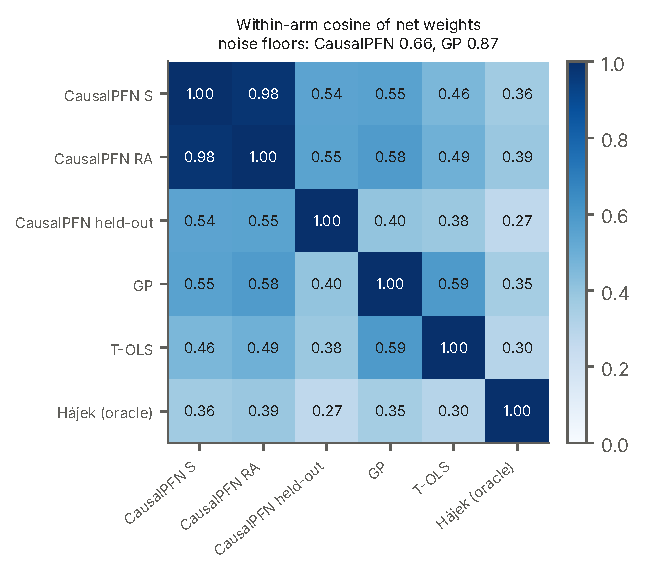
\includegraphics[width=\linewidth]{figures/fig3_weight_similarity.pdf}\end{subfigure}\hfill
\begin{subfigure}{0.5\linewidth}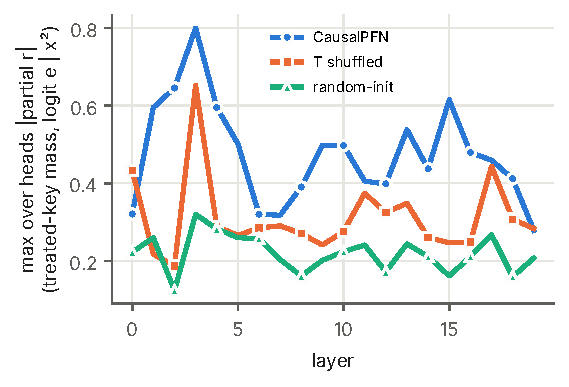
\includegraphics[width=\linewidth]{figures/fig6_attention_propensity.pdf}\end{subfigure}
\caption{Left: mean within-arm cosine between the de-meaned net weights of each pair of estimators (hard DGPs); noise floors are the same estimator after a fresh noise draw. Right: by layer, the maximum over heads of the partial correlation between the attention mass on treated context rows and logit $e$, given a quadratic in $x$, with shuffled-$t$ and random-network controls.}
\end{figure}

\begin{table}[h]
\centering\small
\begin{tabular}{lccc}
\toprule
Estimator & Easy RIC & Hard & Clip \\
\midrule
CausalPFN (S) & \kEasyRic & \kHardPFN & \kClipPFN \\
GP S-learner & 0.984 & \kHardGPfull & \kClipGP \\
AIPW (5-fold) & 0.948 & \kHardAIPW & \kClipAIPW \\
IPW & 0.877 & \kHardIPW & \kClipIPW \\
OLS S-learner & 0.698 & \kHardOLS & 0.487 \\
CausalPFN (held-out) & 0.917 & \kHardHO & 0.575 \\
\bottomrule
\end{tabular}
\caption{Pooled $\kappa$ by suite (20 replications per DGP; all DGPs eligible except 2 in the easy overlap family).}
\end{table}

\end{document}
